% Proposal Fig. 4, slide version: classical branch (Rowley-Brooke, modified; paired photos)
% vs learned branch (DE-GAN, front only). Same conventions as pipeline.tex.
% Build: tectonic bleed/diagrams/comparison.tex
\documentclass[border=8pt]{standalone}
\usepackage{amsmath,amssymb,bm}
\usepackage{tikz}
\usetikzlibrary{shapes.arrows,positioning,shadows,fit,calc}

\definecolor{blockedge}{HTML}{7FA7D9}
\definecolor{navy}{HTML}{1F3B73}
\definecolor{hl}{HTML}{FFF2A8}

\tikzset{
  blk/.style={draw=blockedge, line width=0.9pt, fill=white, text width=6.4cm, minimum height=3.5cm,
              align=center, drop shadow={opacity=0.22, shadow xshift=0.6mm, shadow yshift=-0.6mm}},
  harrow/.style={single arrow, draw=black, fill=white, line width=0.6pt, minimum height=1.05cm,
                 single arrow head extend=0.12cm, inner sep=1.6pt},
}
\newcommand{\ttl}[2]{\textcolor{navy}{\bfseries\Large #1}\\\textcolor{navy}{\bfseries\Large #2}}
\newcommand{\note}[1]{\\[4pt]\mbox{\normalsize\color{black!70}#1}}
\newcommand{\hollow}[2]{%
  \path let \p1=(#1), \p2=(#2), \n1={veclen(\x2-\x1,\y2-\y1)} in
    node[harrow, minimum height=\n1, anchor=tail] at (#1) {};}

\begin{document}
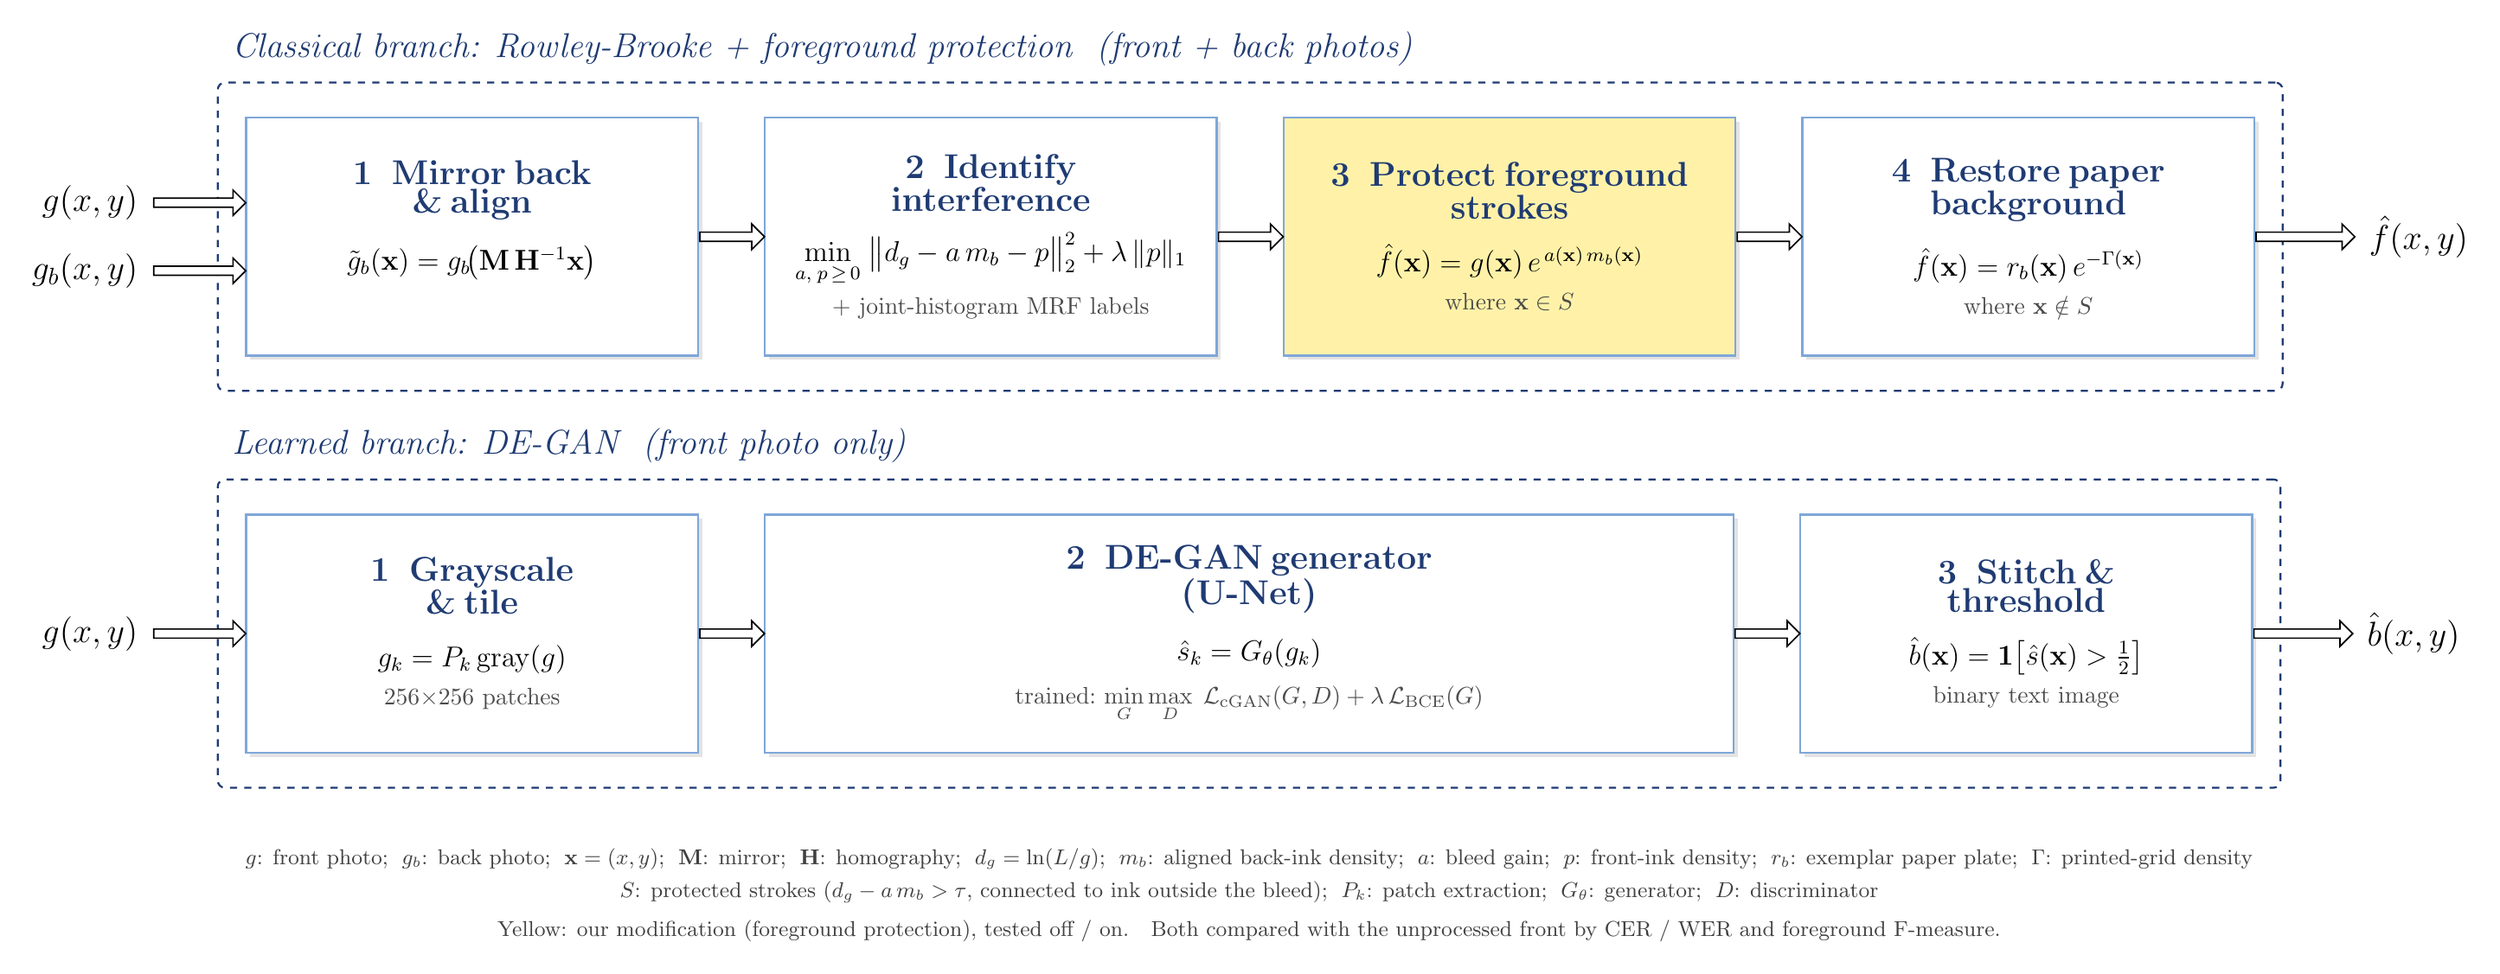
\begin{tikzpicture}[node distance=0.95cm and 0.95cm]
  % ---------------- Classical: Rowley-Brooke, modified ----------------
  \node[blk] (c1) {\ttl{1\enspace Mirror back}{\& align}\\[10pt]
      \mbox{\large$\tilde{g}_b(\mathbf{x}) = g_b\!\bigl(\mathbf{M}\,\mathbf{H}^{-1}\mathbf{x}\bigr)$}
      \note{\phantom{p}}};
  \node[blk, right=of c1] (c2) {\ttl{2\enspace Identify}{interference}\\[8pt]
      \mbox{\large$\displaystyle\min_{a,\;p\,\ge\,0}\;\bigl\lVert d_g - a\,m_b - p\bigr\rVert_2^2 + \lambda\,\lVert p\rVert_1$}
      \note{+ joint-histogram MRF labels}};
  \node[blk, right=of c2, fill=hl] (c3) {\ttl{3\enspace Protect foreground}{strokes}\\[10pt]
      \mbox{\large$\hat{f}(\mathbf{x}) = g(\mathbf{x})\,e^{\,a(\mathbf{x})\,m_b(\mathbf{x})}$}
      \note{where $\mathbf{x}\in S$}};
  \node[blk, right=of c3] (c4) {\ttl{4\enspace Restore paper}{background}\\[10pt]
      \mbox{\large$\hat{f}(\mathbf{x}) = r_b(\mathbf{x})\,e^{-\Gamma(\mathbf{x})}$}
      \note{where $\mathbf{x}\notin S$}};

  % ---------------- Learned: DE-GAN, front only ----------------
  \node[blk, below=2.3cm of c1] (l1) {\ttl{1\enspace Grayscale}{\& tile}\\[10pt]
      \mbox{\large$g_k = P_k\,\mathrm{gray}(g)$}
      \note{256$\times$256 patches}};
  \path (c2.west |- l1) coordinate (l2w);
  \path (c3.east |- l1) coordinate (l2e);
  \node[blk, anchor=west, text width=13.985cm] (l2) at (l2w) {\ttl{2\enspace DE-GAN generator}{(U-Net)}\\[10pt]
      \mbox{\large$\hat{s}_k = G_\theta(g_k)$}\\[6pt]
      \mbox{\normalsize\color{black!70}trained:\ $\displaystyle\min_{G}\max_{D}\;
        \mathcal{L}_{\mathrm{cGAN}}(G,D) + \lambda\,\mathcal{L}_{\mathrm{BCE}}(G)$}};
  \node[blk, right=of l2] (l3) {\ttl{3\enspace Stitch \&}{threshold}\\[10pt]
      \mbox{\large$\hat{b}(\mathbf{x}) = \mathbf{1}\bigl[\hat{s}(\mathbf{x}) > \tfrac12\bigr]$}
      \note{binary text image}};

  % groups
  \node[draw=navy, dashed, line width=0.8pt, rounded corners=3pt, inner xsep=0.4cm, inner ysep=0.5cm,
        fit=(c1)(c4)] (gc) {};
  \node[anchor=south west, font=\itshape\Large, text=navy] at ([xshift=1mm, yshift=1mm]gc.north west)
        {Classical branch: Rowley-Brooke + foreground protection \ (front + back photos)};
  \node[draw=navy, dashed, line width=0.8pt, rounded corners=3pt, inner xsep=0.4cm, inner ysep=0.5cm,
        fit=(l1)(l3)] (gl) {};
  \node[anchor=south west, font=\itshape\Large, text=navy] at ([xshift=1mm, yshift=1mm]gl.north west)
        {Learned branch: DE-GAN \ (front photo only)};

  % inputs / outputs
  \node[anchor=east] (cin1) at ([xshift=-1.45cm, yshift= 0.5cm]c1.west) {\Large $g(x,y)$};
  \node[anchor=east] (cin2) at ([xshift=-1.45cm, yshift=-0.5cm]c1.west) {\Large $g_b(x,y)$};
  \node[anchor=east] (lin)  at ([xshift=-1.45cm]l1.west) {\Large $g(x,y)$};
  \node[anchor=west] (cout) at ([xshift=1.55cm]c4.east) {\Large $\hat{f}(x,y)$};
  \node[anchor=west] (lout) at ([xshift=1.55cm]l3.east) {\Large $\hat{b}(x,y)$};
  \hollow{$(cin1.east)+(0.1,0)$}{$(c1.west|-cin1.east)$}
  \hollow{$(cin2.east)+(0.1,0)$}{$(c1.west|-cin2.east)$}
  \hollow{$(lin.east)+(0.1,0)$}{l1.west}
  \hollow{c1.east}{c2.west}  \hollow{c2.east}{c3.west}  \hollow{c3.east}{c4.west}
  \hollow{c4.east}{$(cout.west)+(-0.1,0)$}
  \hollow{l1.east}{l2.west}  \hollow{l2.east}{l3.west}
  \hollow{l3.east}{$(lout.west)+(-0.1,0)$}

  % key
  \node[below=0.75cm of gl.south, align=center] {%
    {\small\color{black!75}$g$: front photo;\; $g_b$: back photo;\; $\mathbf{x}=(x,y)$;\;
     $\mathbf{M}$: mirror;\; $\mathbf{H}$: homography;\; $d_g=\ln(L/g)$;\; $m_b$: aligned back-ink density;\;
     $a$: bleed gain;\; $p$: front-ink density;\; $r_b$: exemplar paper plate;\; $\Gamma$: printed-grid density}\\[2pt]{\small\color{black!75}$S$: protected strokes ($d_g-a\,m_b>\tau$, connected to ink outside the bleed);\; 
     $P_k$: patch extraction;\; $G_\theta$: generator;\; $D$: discriminator}\\[4pt]
    {\small\color{black!75}Yellow: our modification (foreground protection), tested off / on.\quad
     Both compared with the unprocessed front by CER / WER and foreground F-measure.}};
\end{tikzpicture}
\end{document}
